\chapter{Теория вероятностей: события, условия и независимость}\label{chap:probability}\markright{Глава 46}

\section{Исходы, события и вероятность}
\begin{definition}\term{Пространство элементарных исходов} (\emph{sample space}) \(\Omega\) — множество возможных результатов опыта. \par\term{Событие} (\emph{event}) — допустимое подмножество исходов. В конечной модели допустимы все подмножества \(\Omega\).\end{definition}
\begin{definition}\term{Сигма-алгебра событий} (\emph{sigma-algebra}) \(\mathcal F\) содержит \(\Omega\), дополнения своих элементов и счётные объединения своих элементов. Это точное условие на допустимые события в общей, в том числе непрерывной модели.\end{definition}
\begin{definition}\term{Вероятность} (\emph{probability}) — функция \(\mathbb P\) на событиях, для которой \(\mathbb P(A)\ge0\), \(\mathbb P(\Omega)=1\) и для попарно непересекающихся событий \(\mathbb P(\bigcup_{j=1}^\infty A_j)=\sum_{j=1}^\infty\mathbb P(A_j)\). \par\term{Вероятностное пространство} (\emph{probability space}) — тройка \((\Omega,\mathcal F,\mathbb P)\), удовлетворяющая указанным условиям.\end{definition}
\par\addvspace{5pt}\begin{lrbox}{\CatFlowBox}\begin{minipage}[t]{\linewidth}
\setlength{\parskip}{5pt}\setlength{\columnsep}{4.5mm}\setlength{\intextsep}{0pt}
\begin{wrapfigure}[11]{r}{54mm}
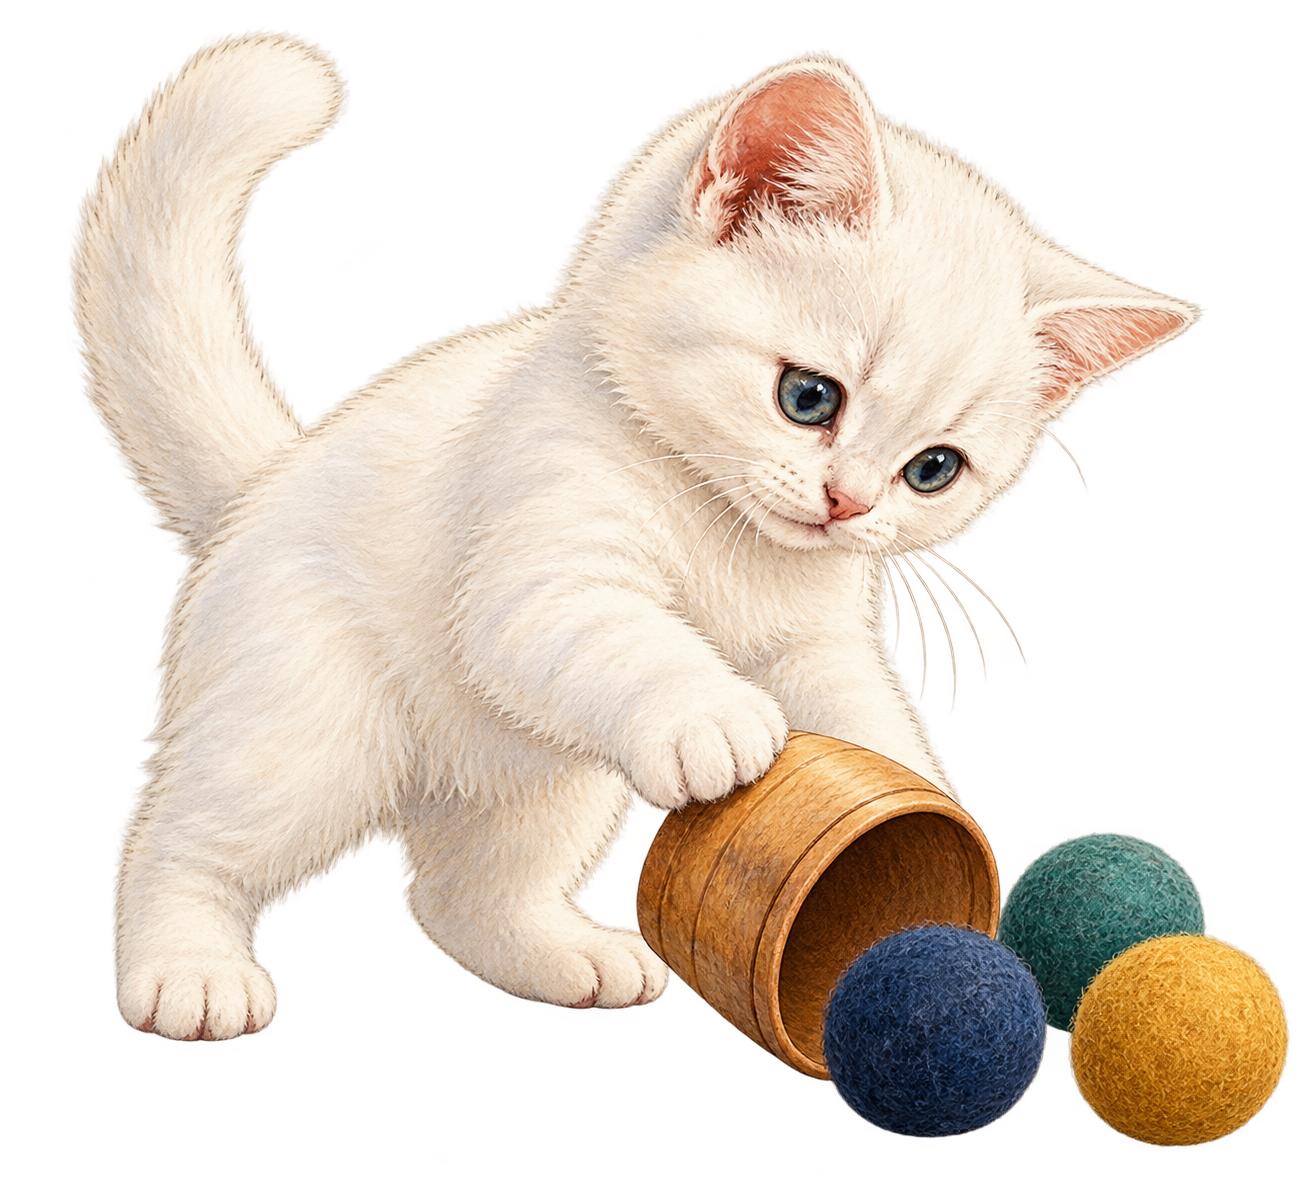
\includegraphics[width=54mm,height=58mm,keepaspectratio]{images/unique/art-166.png}
\end{wrapfigure}
Случайность описывается моделью, а не одним списком возможных ответов. При броске двух честных кубиков равновероятны 36 упорядоченных пар, а не 11 возможных сумм. Сумма \(7\) встречается чаще суммы \(2\), потому что ей соответствует больше пар. Формула «благоприятные исходы, делённые на все исходы» применима только после проверки равновероятности.
\par\WFclear\end{minipage}\end{lrbox}%
\ifdim\dimexpr\ht\CatFlowBox+\dp\CatFlowBox\relax<64mm\dp\CatFlowBox=\dimexpr64mm-\ht\CatFlowBox\relax\fi%
\noindent\usebox{\CatFlowBox}\par\addvspace{5pt}
\begin{definition}\term{Классическая конечная модель} (\emph{equally likely finite model}) имеет \(N\) равновероятных исходов: \(\mathbb P(A)=\frac{|A|}{N}\). \par\term{Противоположное событие} (\emph{complementary event}) \(A^c=\Omega\setminus A\).\end{definition}
\begin{theorem}[Следствия аксиом вероятности]
\(\mathbb P(\varnothing)=0\), \(0\le\mathbb P(A)\le1\), \(\mathbb P(A^c)=1-\mathbb P(A)\). Если \(A\subseteq B\), то \(\mathbb P(A)\le\mathbb P(B)\). Для любых \(A,B\)
\[
\mathbb P(A\cup B)=\mathbb P(A)+\mathbb P(B)-\mathbb P(A\cap B).
\]
\end{theorem}
\begin{proof}Из разбиения \(\Omega=\Omega\cup\varnothing\) на непересекающиеся части следует \(\mathbb P(\varnothing)=0\). Разбиение \(\Omega=A\cup A^c\) даёт формулу дополнения и границы. Для \(A\subseteq B\) пишем \(B=A\cup(B\setminus A)\). Для последней формулы разбиваем \(A\cup B\) на \(A\setminus B,A\cap B,B\setminus A\); пересечение в сумме \(\mathbb P(A)+\mathbb P(B)\) было посчитано дважды.\end{proof}
\begin{theorem}[Оценка объединения; union bound]
Для конечного числа событий \(\mathbb P(\bigcup_{j=1}^m A_j)\le\sum_{j=1}^m\mathbb P(A_j)\); независимость не требуется.
\end{theorem}
\begin{proof}Для двух событий вычитаем неотрицательную вероятность пересечения из предыдущей формулы. Для большего числа применяем это неравенство по индукции.\end{proof}
\section{Условная вероятность и формула Байеса}
\begin{definition}\term{Условная вероятность} (\emph{conditional probability}) при \(\mathbb P(B)>0\) определяется как \(\mathbb P(A\mid B)=\frac{\mathbb P(A\cap B)}{\mathbb P(B)}\).\end{definition}
\begin{theorem}[Правило умножения]
При \(\mathbb P(B)>0\): \(\mathbb P(A\cap B)=\mathbb P(B)\mathbb P(A\mid B)\). Для последовательных условий формула повторяется, если все используемые условные вероятности определены.
\end{theorem}
\par\addvspace{5pt}\begin{lrbox}{\CatFlowBox}\begin{minipage}[t]{\linewidth}
\setlength{\parskip}{5pt}\setlength{\columnsep}{4.5mm}\setlength{\intextsep}{0pt}
\begin{wrapfigure}[9]{l}{54mm}
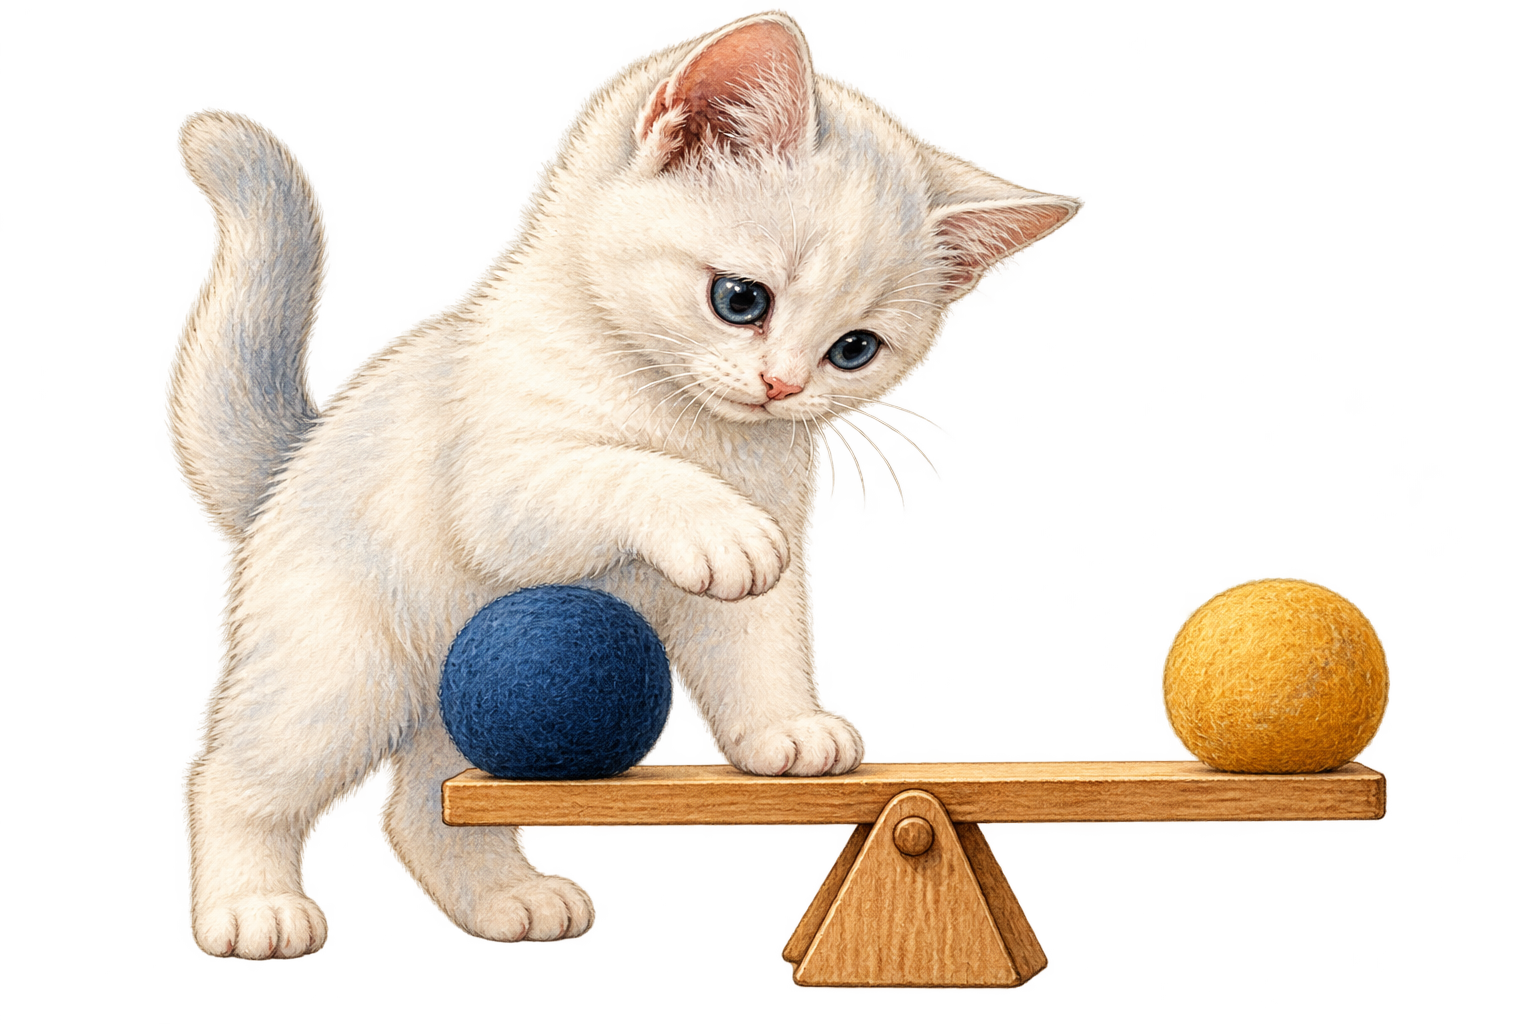
\includegraphics[width=54mm,height=58mm,keepaspectratio]{images/unique/art-169.png}
\end{wrapfigure}
\textit{Доказательство.} Умножаем определение условной вероятности на знаменатель. Следующее применение берёт уже накопленное пересечение как условие.\hfill\(\blacksquare\)
\par\WFclear\end{minipage}\end{lrbox}%
\ifdim\dimexpr\ht\CatFlowBox+\dp\CatFlowBox\relax<64mm\dp\CatFlowBox=\dimexpr64mm-\ht\CatFlowBox\relax\fi%
\noindent\usebox{\CatFlowBox}\par\addvspace{5pt}

\begin{definition}\term{Полная группа событий} (\emph{partition of the sample space}) \(B_1,\ldots,B_m\) состоит из попарно непересекающихся событий, объединение которых равно \(\Omega\).\end{definition}
\begin{theorem}[Полная вероятность и Байес; total probability and Bayes' formula]
Для полной группы с \(\mathbb P(B_j)>0\)
\[
\mathbb P(A)=\sum_{j=1}^m\mathbb P(B_j)\mathbb P(A\mid B_j).
\]
Если также \(\mathbb P(A)>0\), то
\[
\mathbb P(B_k\mid A)=
\frac{\mathbb P(B_k)\mathbb P(A\mid B_k)}
{\sum_{j=1}^m\mathbb P(B_j)\mathbb P(A\mid B_j)}.
\]
\end{theorem}
\begin{proof}Событие \(A\) разбивается на непересекающиеся \(A\cap B_j\). Складываем вероятности и применяем правило умножения. Для Байеса записываем \(\mathbb P(B_k\mid A)=\frac{\mathbb P(A\cap B_k)}{\mathbb P(A)}\) и подставляем уже найденные числитель и знаменатель.\end{proof}
\par\addvspace{5pt}\begin{lrbox}{\CatFlowBox}\begin{minipage}[t]{\linewidth}
\setlength{\parskip}{5pt}\setlength{\columnsep}{4.5mm}\setlength{\intextsep}{0pt}
\begin{wrapfigure}[11]{l}{54mm}
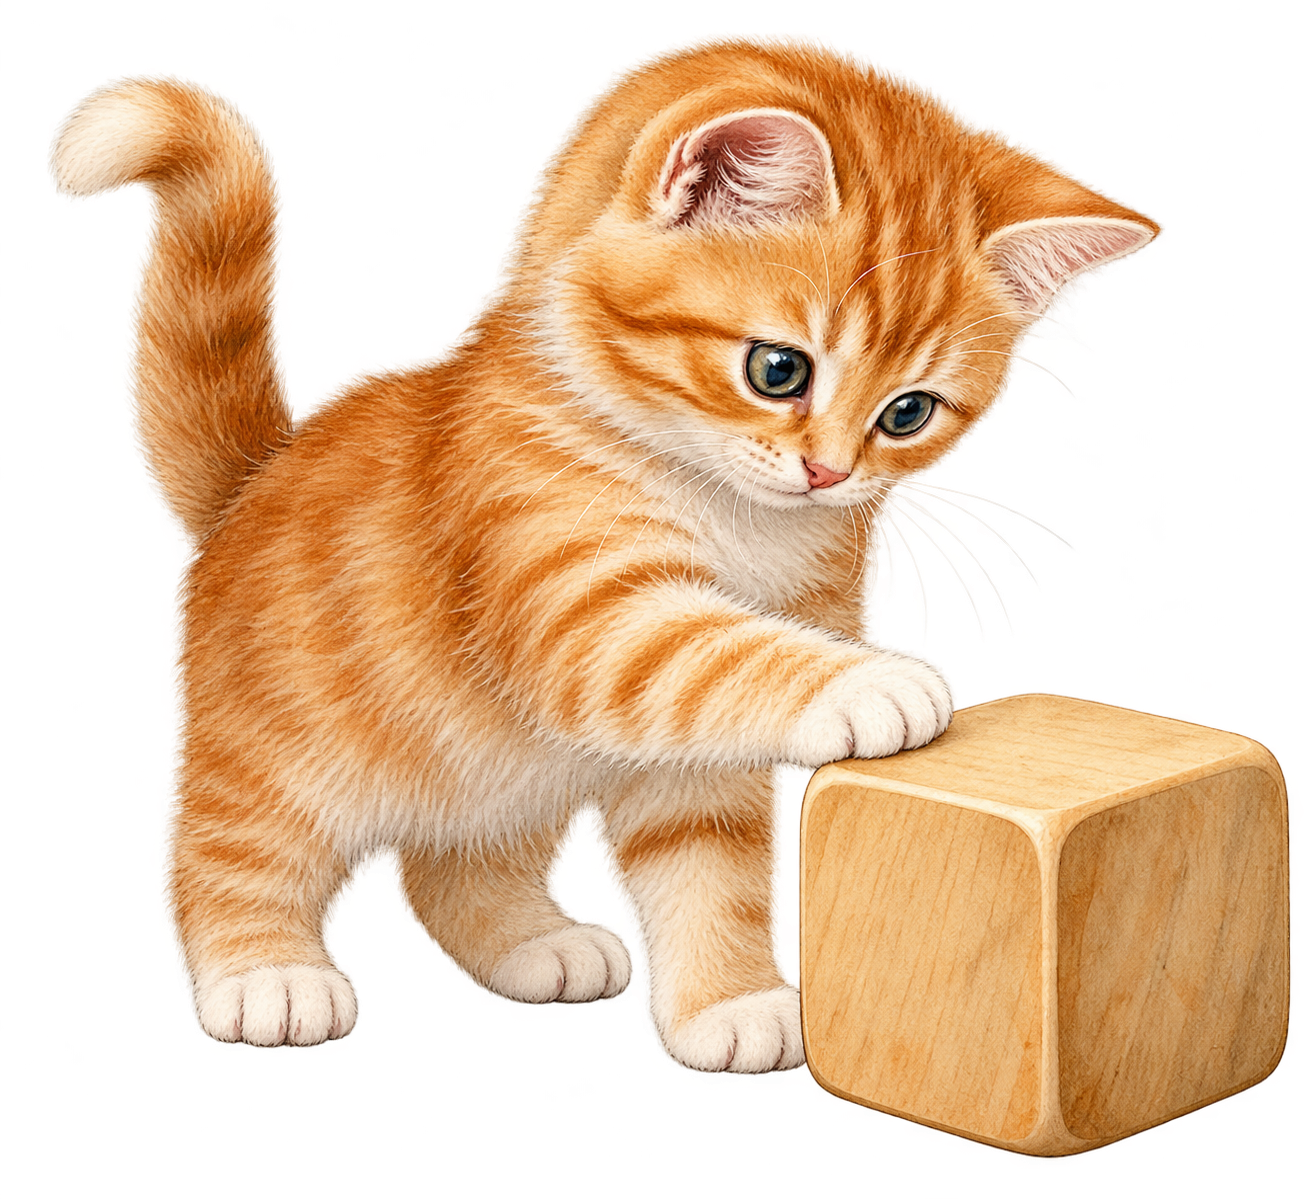
\includegraphics[width=54mm,height=58mm,keepaspectratio]{images/unique/art-167.png}
\end{wrapfigure}
Формула Байеса меняет направление условного вопроса. Доля красных шаров в выбранном мешке и вероятность выбрать именно этот мешок после появления красного шара — разные числа. До наблюдения важны доли выбора мешков; после наблюдения остаются только исходы, согласованные с увиденным цветом. Поэтому редкий источник не становится наиболее вероятным автоматически, даже если в нём нужный цвет встречается часто.
\par\WFclear\end{minipage}\end{lrbox}%
\ifdim\dimexpr\ht\CatFlowBox+\dp\CatFlowBox\relax<64mm\dp\CatFlowBox=\dimexpr64mm-\ht\CatFlowBox\relax\fi%
\noindent\usebox{\CatFlowBox}\par\addvspace{5pt}
\section{Независимость и повторные испытания}
\begin{definition}\term{Независимость двух событий} (\emph{independence}) означает \(\mathbb P(A\cap B)=\mathbb P(A)\mathbb P(B)\). При \(\mathbb P(B)>0\) это равносильно \(\mathbb P(A\mid B)=\mathbb P(A)\).\end{definition}
\begin{definition}\term{Независимость в совокупности} (\emph{mutual independence}) событий \(A_1,\ldots,A_n\) требует равенства вероятности пересечения произведению вероятностей для каждого непустого поднабора. Одной попарной независимости для \(n\ge3\) недостаточно.\end{definition}
\par\addvspace{5pt}\begin{lrbox}{\CatFlowBox}\begin{minipage}[t]{\linewidth}
\setlength{\parskip}{5pt}\setlength{\columnsep}{4.5mm}\setlength{\intextsep}{0pt}
\begin{wrapfigure}[11]{r}{54mm}
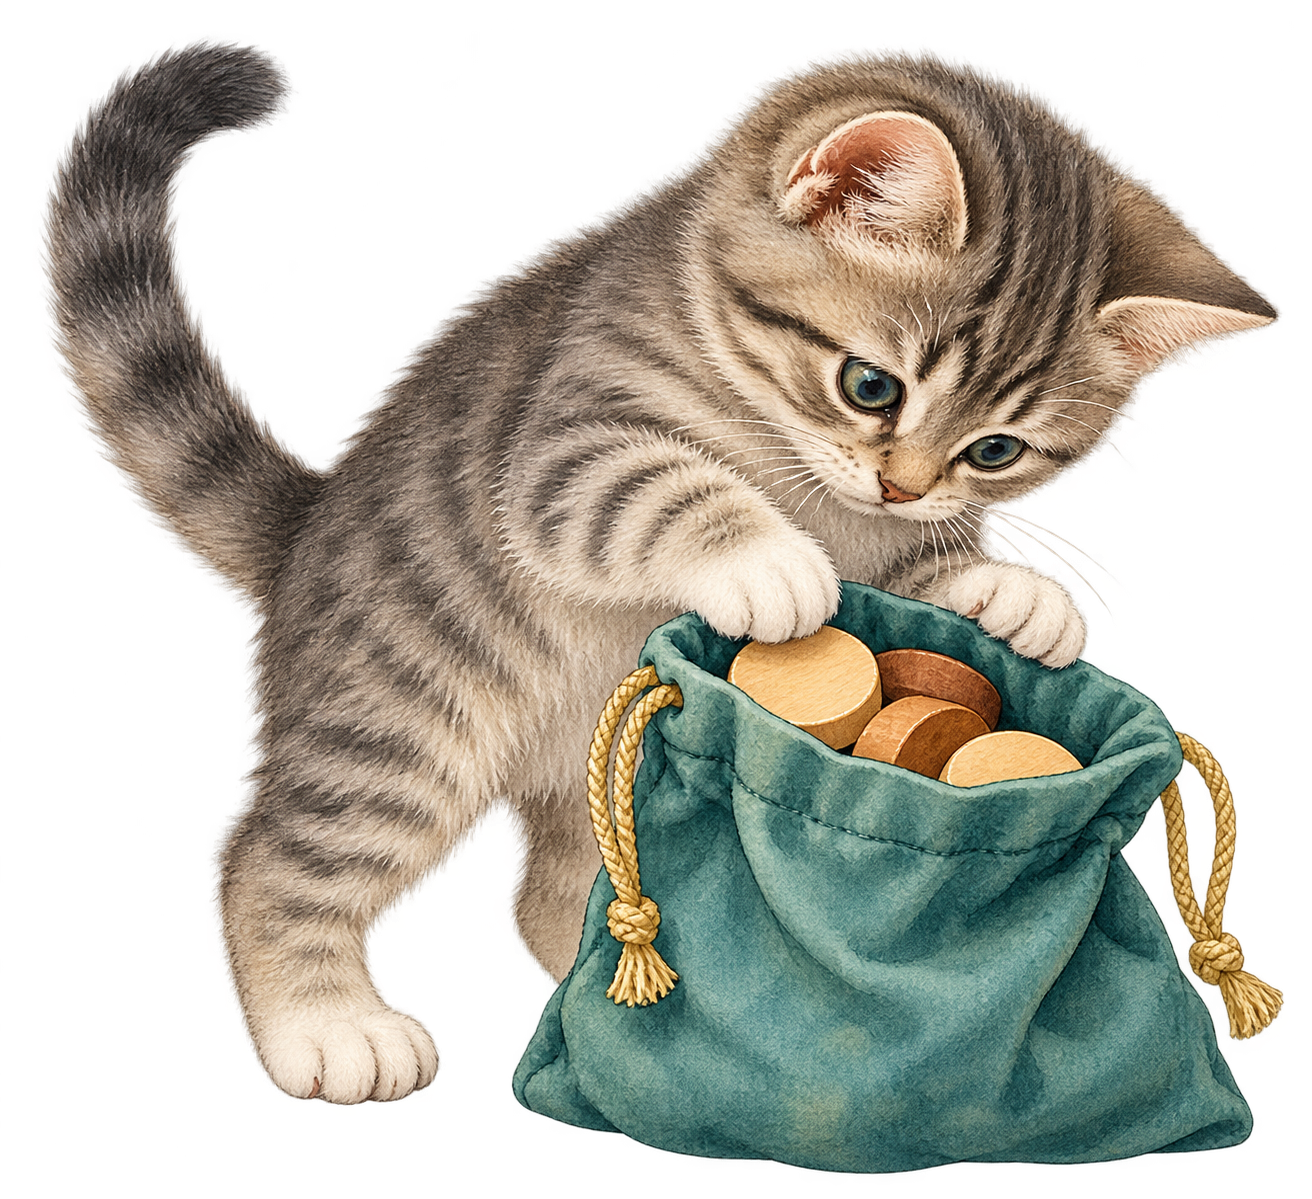
\includegraphics[width=54mm,height=58mm,keepaspectratio]{images/unique/art-168.png}
\end{wrapfigure}
Несовместность и независимость отвечают на разные вопросы. Несовместные события не могут случиться вместе; независимые не меняют вероятностей друг друга при условии положительной вероятности условия. Если два несовместных события оба имеют положительную вероятность, они зависимы. Независимость повторных опытов должна быть частью модели: вытаскивание шаров без возвращения обычно её нарушает.
\par\WFclear\end{minipage}\end{lrbox}%
\ifdim\dimexpr\ht\CatFlowBox+\dp\CatFlowBox\relax<64mm\dp\CatFlowBox=\dimexpr64mm-\ht\CatFlowBox\relax\fi%
\noindent\usebox{\CatFlowBox}\par\addvspace{5pt}
\begin{definition}\term{Схема Бернулли} (\emph{Bernoulli trials}) — \(n\) независимых в совокупности испытаний, в каждом из которых успех имеет одну вероятность \(p\), а неуспех \(1-p\).\end{definition}
\begin{theorem}[Число успехов в схеме Бернулли]
При \(0<p<1\) вероятность ровно \(k\) успехов, \(0\le k\le n\), равна
\[
\binom nk p^k(1-p)^{n-k}.
\]
При \(p=0\) успехов всегда \(0\); при \(p=1\) их всегда \(n\).
\end{theorem}
\begin{proof}Фиксированная последовательность из \(k\) успехов и \(n-k\) неуспехов имеет указанное произведение вероятностей по независимости. Выбрать позиции успехов можно \(\binom nk\) способами; эти события не пересекаются. Складываем их вероятности. Граничные случаи детерминированы, поэтому выражения с неопределённой записью \(0^0\) не требуются.\end{proof}

\section{Примеры: выбор без возвращения и Байес}
\begin{example}В коробке три красных и два синих шара. Равномерно извлекают два по очереди без возвращения. Вероятность двух красных равна \(\frac35\cdot\frac24=\frac3{10}\). Второй множитель --- условная вероятность после первого красного; независимости нет. Тот же ответ по сочетаниям: \(\frac{C_3^2}{C_5^2}=\frac3{10}\).\end{example}
\begin{example}Станок A производит \(60\%\) деталей, B --- \(40\%\). Доли брака \(2\%\) и \(5\%\) соответственно. Выбирают равномерно деталь из общего большого выпуска с указанными долями. Вероятность брака \(0{,}6\cdot0{,}02+0{,}4\cdot0{,}05=0{,}032\). Если выбранная деталь оказалась бракованной, вероятность происхождения из A равна \(\frac{0{,}6\cdot0{,}02}{0{,}032}=\frac38\). Условие о браке меняет веса источников.\end{example}
\par\noindent\begin{minipage}{\linewidth}\section*{Графики}
\begin{center}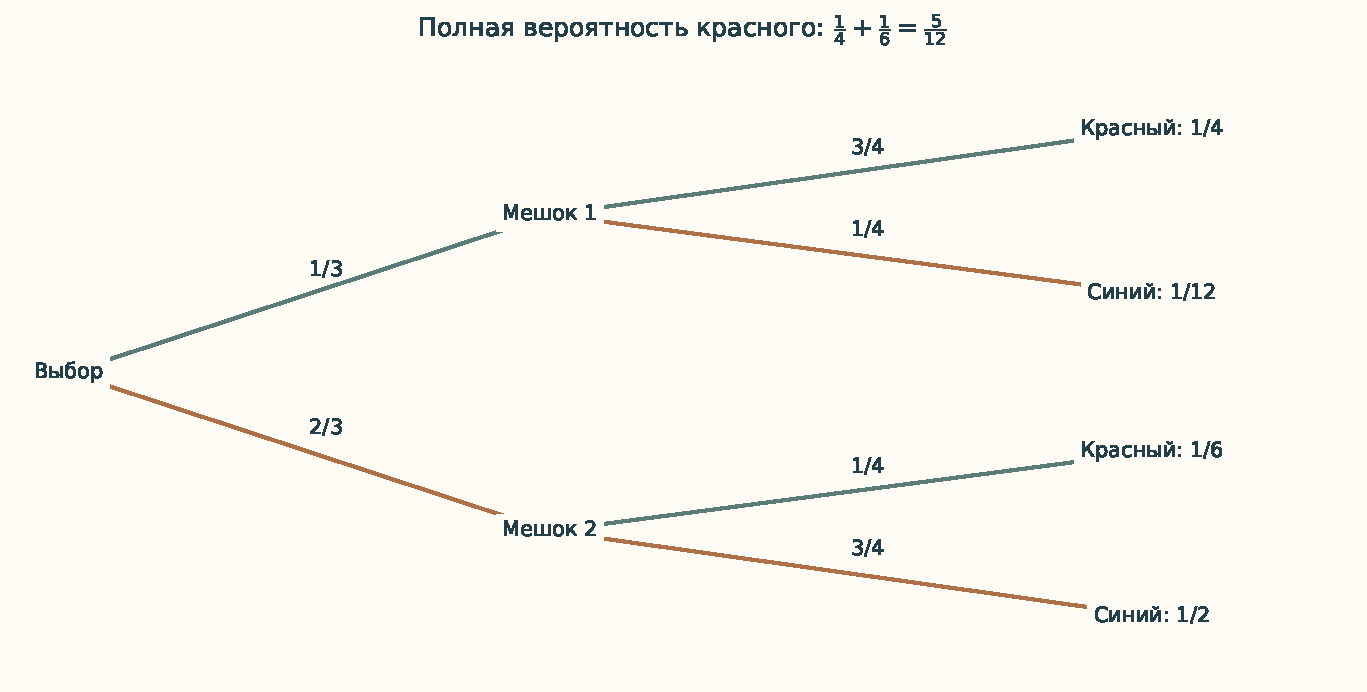
\includegraphics[width=\textwidth,height=.79\textheight,keepaspectratio]{images/atlas-probability.pdf}\par\small Дерево условных вероятностей\end{center}\end{minipage}\par
\Needspace{7\baselineskip}\section*{Задачи}
\begingroup\setlength{\parskip}{1pt}
\noindent\begin{minipage}[t]{\linewidth}\textbf{46.1.} Два честных кубика бросают независимо. Опиши равновероятные исходы и найди вероятность суммы \(7\).\par\end{minipage}\par
\noindent\begin{minipage}[t]{\linewidth}\textbf{46.2.} На честном кубике найди вероятность чётного результата.\par\end{minipage}\par
\noindent\begin{minipage}[t]{\linewidth}\textbf{46.3.} Из \(10\) одинаковых на ощупь жетонов, \(4\) из которых синие, равновероятно выбирают один. Найди вероятность синего и несинего.\par\end{minipage}\par
\noindent\begin{minipage}[t]{\linewidth}\textbf{46.4.} Даны \(\mathbb P(A)=0{,}6\), \(\mathbb P(B)=0{,}5\), \(\mathbb P(A\cap B)=0{,}2\). Найди вероятность хотя бы одного и вероятность ни одного.\par\end{minipage}\par
\noindent\begin{minipage}[t]{\linewidth}\textbf{46.5.} Могут ли несовместные события с положительными вероятностями быть независимыми?\par\end{minipage}\par
\par\addvspace{5pt}\begin{lrbox}{\CatFlowBox}\begin{minipage}[t]{\linewidth}
\setlength{\parskip}{5pt}\setlength{\columnsep}{4.5mm}\setlength{\intextsep}{0pt}
\begin{wrapfigure}[12]{r}{54mm}
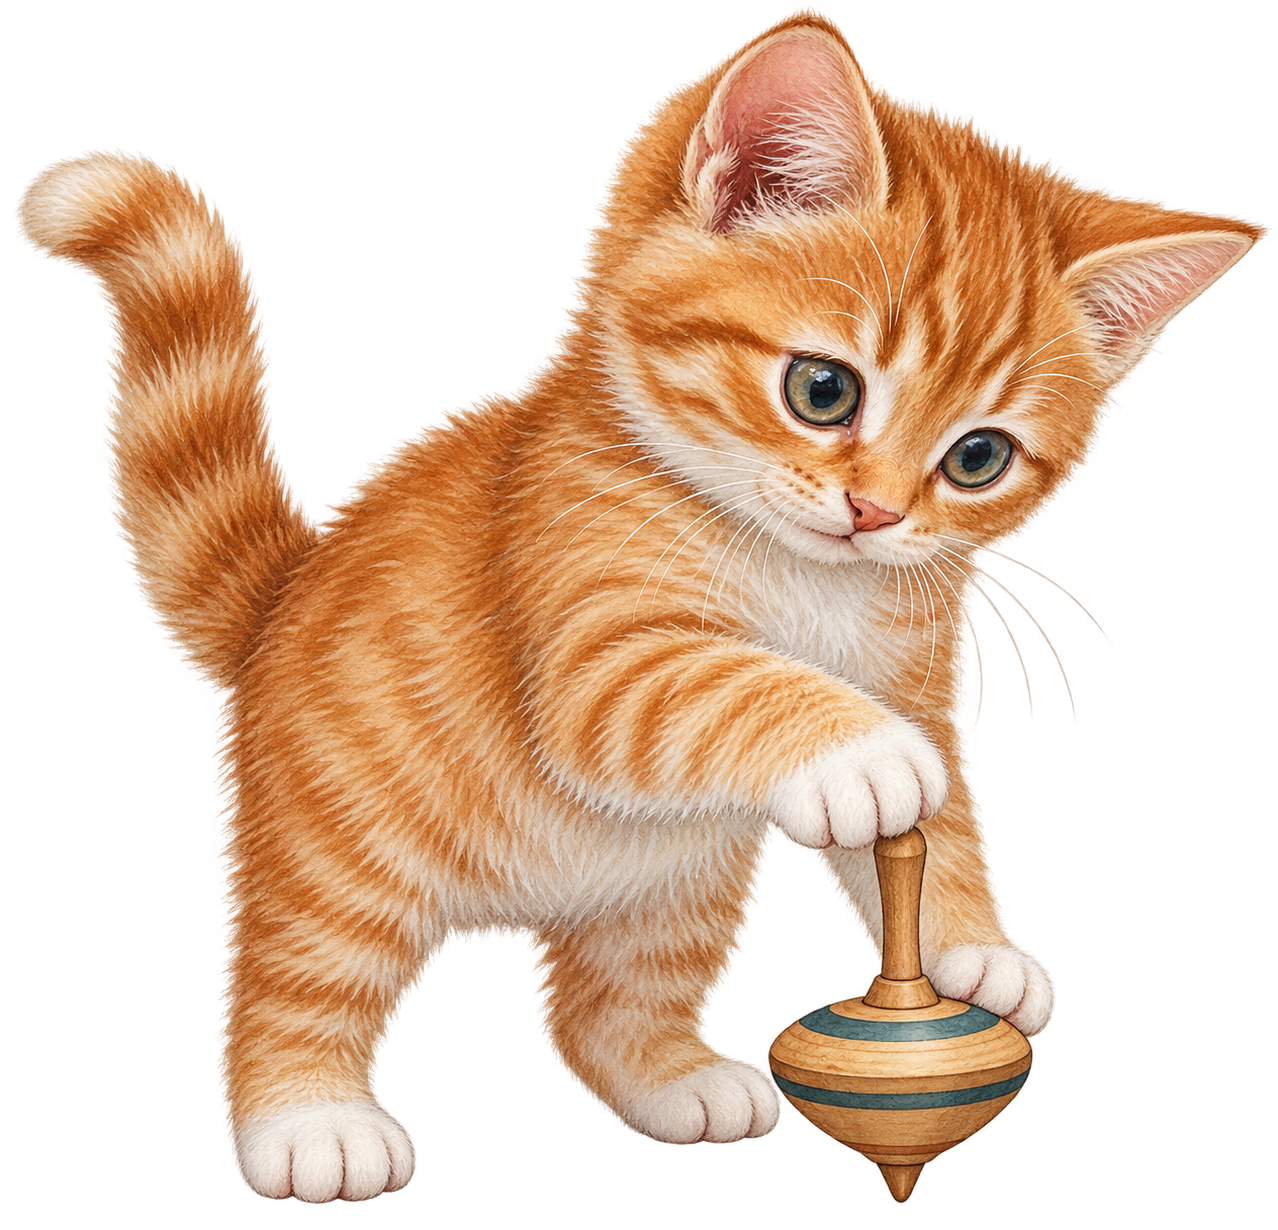
\includegraphics[width=54mm,height=58mm,keepaspectratio]{images/unique/art-170.png}
\end{wrapfigure}
\textbf{46.6.} Независимые события имеют вероятности \(0{,}3\) и \(0{,}4\). Найди вероятность обоих и хотя бы одного.\par

\textbf{46.7.} Честный кубик показал число больше \(3\). Найди условную вероятность чётного результата.\par

\textbf{46.8.} В мешке \(3\) красных и \(2\) синих шара. Извлекают два без возвращения. Найди вероятность двух красных. На каждом извлечении все оставшиеся в мешке шары равновероятны.\par

\textbf{46.9.} В том же мешке первый шар оказался красным. Найди вероятность красного второго и сравни с его безусловной вероятностью. На каждом извлечении все оставшиеся в мешке шары равновероятны.\par
\par\WFclear\end{minipage}\end{lrbox}%
\ifdim\dimexpr\ht\CatFlowBox+\dp\CatFlowBox\relax<64mm\dp\CatFlowBox=\dimexpr64mm-\ht\CatFlowBox\relax\fi%
\noindent\usebox{\CatFlowBox}\par\addvspace{5pt}

\noindent\begin{minipage}[t]{\linewidth}\textbf{46.10.} В мешке \(3\) красных и \(2\) синих шара. Два раза выбирают шар, возвращая и перемешивая его после первого выбора. Найди вероятность ровно одного красного. На каждом извлечении все оставшиеся в мешке шары равновероятны.\par\end{minipage}\par
\noindent\begin{minipage}[t]{\linewidth}\textbf{46.11.} Первый мешок выбирают с вероятностью \(\dfrac13\), второй — \(\dfrac23\). Доли красных шаров в них \(\dfrac34,\dfrac14\). После случайного извлечения получен красный. Найди вероятность первого мешка.\par\end{minipage}\par
\noindent\begin{minipage}[t]{\linewidth}\textbf{46.12.} В учебной модели первая линия выпускает \(70\%\) деталей с долей дефектов \(2\%\), вторая \(30\%\) с долей \(5\%\). Найди общую вероятность дефекта и вероятность второй линии при обнаруженном дефекте.\par\end{minipage}\par
\noindent\begin{minipage}[t]{\linewidth}\textbf{46.13.} В трёх независимых бросках честной монеты найди вероятность ровно двух орлов.\par\end{minipage}\par
\noindent\begin{minipage}[t]{\linewidth}\textbf{46.14.} В четырёх независимых бросках честной монеты найди вероятность хотя бы одного орла.\par\end{minipage}\par
\noindent\begin{minipage}[t]{\linewidth}\textbf{46.15.} В пяти испытаниях Бернулли \(p=\dfrac15\). Найди вероятность отсутствия успехов.\par\end{minipage}\par
\noindent\begin{minipage}[t]{\linewidth}\textbf{46.16.} Независимые попытки имеют вероятность успеха \(\dfrac14\). Найди вероятность первого успеха на третьей попытке.\par\end{minipage}\par
\noindent\begin{minipage}[t]{\linewidth}\textbf{46.17.} Из \(6\) человек равновероятно выбирают команду из \(3\). Найди вероятность попадания в неё двух заранее указанных людей.\par\end{minipage}\par
\noindent\begin{minipage}[t]{\linewidth}\textbf{46.18.} Число равновероятно выбирают из \(1,\ldots,100\). Найди вероятность делимости на \(3\) или \(5\).\par\end{minipage}\par
\noindent\begin{minipage}[t]{\linewidth}\textbf{46.19.}\starmark{} Две честные монеты бросают независимо. События: \(A\) — орёл на первой, \(B\) — орёл на второй, \(C\) — результаты совпали. Докажи попарную независимость и отсутствие независимости в совокупности.\par\end{minipage}\par
\noindent\begin{minipage}[t]{\linewidth}\textbf{46.20.} У каждого из трёх датчиков вероятность отказа не больше \(0{,}02\). Независимость не дана. Оцени снизу вероятность, что все исправны.\par\end{minipage}\par
\noindent\begin{minipage}[t]{\linewidth}\textbf{46.21.}\starmark{} Докажи, что при фиксированном \(B\) положительной вероятности функция \(A\mapsto\mathbb P(A\mid B)\) удовлетворяет аксиомам вероятности.\par\end{minipage}\par
\noindent\begin{minipage}[t]{\linewidth}\textbf{46.22.} Выведи \(\mathbb P(A\mid B)\mathbb P(B)=\mathbb P(B\mid A)\mathbb P(A)\), указав условия определённости обеих условных вероятностей.\par\end{minipage}\par
\noindent\begin{minipage}[t]{\linewidth}\textbf{46.23.}\starmark{} Три честных кубика бросают независимо. Найди вероятность суммы \(4\).\par\end{minipage}\par
\noindent\begin{minipage}[t]{\linewidth}\textbf{46.24.}\starmark{} Независимые \(A,B\) имеют вероятности \(p,q\), причём \(p+q-pq>0\). Вырази \(\mathbb P(A\mid A\cup B)\).\par\end{minipage}\par
\endgroup
